\documentclass[twoside]{book}

% Packages required by doxygen
\usepackage{fixltx2e}
\usepackage{calc}
\usepackage{doxygen}
\usepackage[export]{adjustbox} % also loads graphicx
\usepackage{graphicx}
\usepackage[utf8]{inputenc}
\usepackage{makeidx}
\usepackage{multicol}
\usepackage{multirow}
\PassOptionsToPackage{warn}{textcomp}
\usepackage{textcomp}
\usepackage[nointegrals]{wasysym}
\usepackage[table]{xcolor}

% Font selection
\usepackage[T1]{fontenc}
\usepackage[scaled=.90]{helvet}
\usepackage{courier}
\usepackage{amssymb}
\usepackage{sectsty}
\renewcommand{\familydefault}{\sfdefault}
\allsectionsfont{%
  \fontseries{bc}\selectfont%
  \color{darkgray}%
}
\renewcommand{\DoxyLabelFont}{%
  \fontseries{bc}\selectfont%
  \color{darkgray}%
}
\newcommand{\+}{\discretionary{\mbox{\scriptsize$\hookleftarrow$}}{}{}}

% Page & text layout
\usepackage{geometry}
\geometry{%
  a4paper,%
  top=2.5cm,%
  bottom=2.5cm,%
  left=2.5cm,%
  right=2.5cm%
}
\tolerance=750
\hfuzz=15pt
\hbadness=750
\setlength{\emergencystretch}{15pt}
\setlength{\parindent}{0cm}
\setlength{\parskip}{3ex plus 2ex minus 2ex}
\makeatletter
\renewcommand{\paragraph}{%
  \@startsection{paragraph}{4}{0ex}{-1.0ex}{1.0ex}{%
    \normalfont\normalsize\bfseries\SS@parafont%
  }%
}
\renewcommand{\subparagraph}{%
  \@startsection{subparagraph}{5}{0ex}{-1.0ex}{1.0ex}{%
    \normalfont\normalsize\bfseries\SS@subparafont%
  }%
}
\makeatother

% Headers & footers
\usepackage{fancyhdr}
\pagestyle{fancyplain}
\fancyhead[LE]{\fancyplain{}{\bfseries\thepage}}
\fancyhead[CE]{\fancyplain{}{}}
\fancyhead[RE]{\fancyplain{}{\bfseries\leftmark}}
\fancyhead[LO]{\fancyplain{}{\bfseries\rightmark}}
\fancyhead[CO]{\fancyplain{}{}}
\fancyhead[RO]{\fancyplain{}{\bfseries\thepage}}
\fancyfoot[LE]{\fancyplain{}{}}
\fancyfoot[CE]{\fancyplain{}{}}
\fancyfoot[RE]{\fancyplain{}{\bfseries\scriptsize Generated by Doxygen }}
\fancyfoot[LO]{\fancyplain{}{\bfseries\scriptsize Generated by Doxygen }}
\fancyfoot[CO]{\fancyplain{}{}}
\fancyfoot[RO]{\fancyplain{}{}}
\renewcommand{\footrulewidth}{0.4pt}
\renewcommand{\chaptermark}[1]{%
  \markboth{#1}{}%
}
\renewcommand{\sectionmark}[1]{%
  \markright{\thesection\ #1}%
}

% Indices & bibliography
\usepackage{natbib}
\usepackage[titles]{tocloft}
\setcounter{tocdepth}{3}
\setcounter{secnumdepth}{5}
\makeindex

% Hyperlinks (required, but should be loaded last)
\usepackage{ifpdf}
\ifpdf
  \usepackage[pdftex,pagebackref=true]{hyperref}
\else
  \usepackage[ps2pdf,pagebackref=true]{hyperref}
\fi
\hypersetup{%
  colorlinks=true,%
  linkcolor=blue,%
  citecolor=blue,%
  unicode%
}

% Custom commands
\newcommand{\clearemptydoublepage}{%
  \newpage{\pagestyle{empty}\cleardoublepage}%
}

\usepackage{caption}
\captionsetup{labelsep=space,justification=centering,font={bf},singlelinecheck=off,skip=4pt,position=top}

%===== C O N T E N T S =====

\begin{document}

% Titlepage & ToC
\hypersetup{pageanchor=false,
             bookmarksnumbered=true,
             pdfencoding=unicode
            }
\pagenumbering{roman}
\begin{titlepage}
\vspace*{7cm}
\begin{center}%
{\Large J\+P\+C\+R\+E2 \\[1ex]\large 10.\+25.\+01 }\\
\vspace*{1cm}
{\large Generated by Doxygen 1.8.11}\\
\end{center}
\end{titlepage}
\clearemptydoublepage
\tableofcontents
\clearemptydoublepage
\pagenumbering{arabic}
\hypersetup{pageanchor=true}

%--- Begin generated contents ---
\chapter{File Index}
\section{File List}
Here is a list of all documented files with brief descriptions\+:\begin{DoxyCompactList}
\item\contentsline{section}{\hyperlink{jpcre2_8hpp}{jpcre2.\+hpp} \\*Main header file for J\+P\+C\+RE library to be included by programs that call J\+P\+C\+R\+E2 functions }{\pageref{jpcre2_8hpp}}{}
\end{DoxyCompactList}

\chapter{File Documentation}
\hypertarget{jpcre2_8cpp}{}\subsection{jpcre2.\+cpp File Reference}
\label{jpcre2_8cpp}\index{jpcre2.\+cpp@{jpcre2.\+cpp}}
{\ttfamily \#include \char`\"{}jpcre2.\+hpp\char`\"{}}\newline
{\ttfamily \#include $<$cstdio$>$}\newline
{\ttfamily \#include $<$limits$>$}\newline
{\ttfamily \#include $<$cassert$>$}\newline
{\ttfamily \#include $<$cstring$>$}\newline
Include dependency graph for jpcre2.\+cpp\+:\nopagebreak
\begin{figure}[H]
\begin{center}
\leavevmode
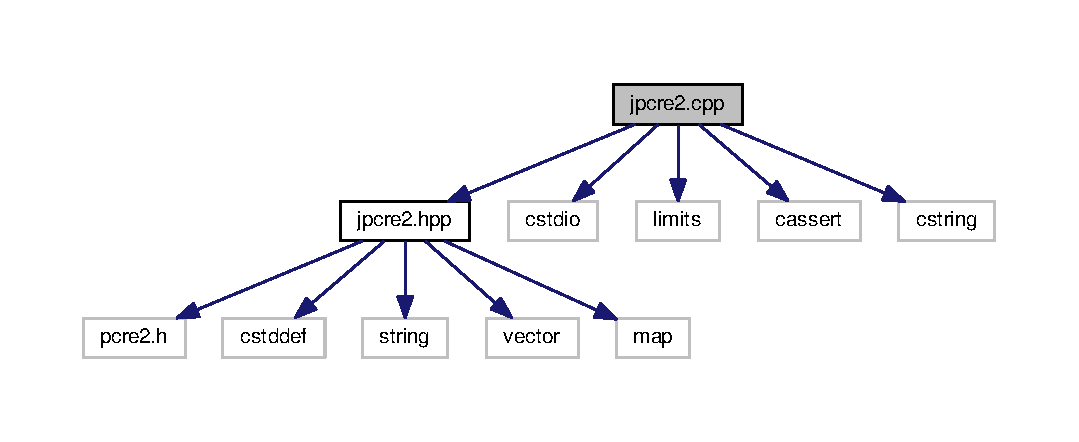
\includegraphics[width=350pt]{jpcre2_8cpp__incl}
\end{center}
\end{figure}

\hypertarget{jpcre2_8hpp}{}\section{jpcre2.\+hpp File Reference}
\label{jpcre2_8hpp}\index{jpcre2.\+hpp@{jpcre2.\+hpp}}


Main header file for J\+P\+C\+RE library to be included by programs that call J\+P\+C\+R\+E2 functions.  


{\ttfamily \#include $<$pcre2.\+h$>$}\\*
{\ttfamily \#include $<$stdint.\+h$>$}\\*
{\ttfamily \#include $<$cstddef$>$}\\*
{\ttfamily \#include $<$string$>$}\\*
{\ttfamily \#include $<$vector$>$}\\*
{\ttfamily \#include $<$map$>$}\\*
Include dependency graph for jpcre2.\+hpp\+:\nopagebreak
\begin{figure}[H]
\begin{center}
\leavevmode
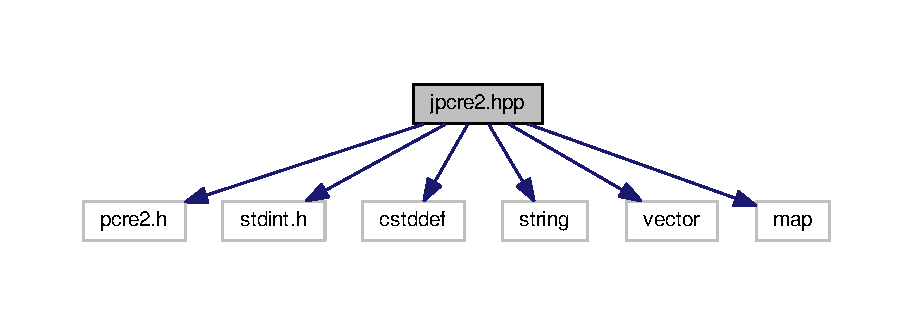
\includegraphics[width=350pt]{jpcre2_8hpp__incl}
\end{center}
\end{figure}
\subsection*{Classes}
\begin{DoxyCompactItemize}
\item 
class \hyperlink{classjpcre2_1_1RegexMatch}{jpcre2\+::\+Regex\+Match}
\begin{DoxyCompactList}\small\item\em Performs regex matching. \end{DoxyCompactList}\item 
class \hyperlink{classjpcre2_1_1RegexReplace}{jpcre2\+::\+Regex\+Replace}
\begin{DoxyCompactList}\small\item\em Performs regex replace on a string. \end{DoxyCompactList}\item 
class \hyperlink{classjpcre2_1_1Regex}{jpcre2\+::\+Regex}
\begin{DoxyCompactList}\small\item\em This is the main class that is to be used to perform all J\+P\+C\+R\+E2 related actions. \end{DoxyCompactList}\end{DoxyCompactItemize}
\subsection*{Namespaces}
\begin{DoxyCompactItemize}
\item 
 \hyperlink{namespacejpcre2}{jpcre2}
\begin{DoxyCompactList}\small\item\em Main namespace of J\+P\+C\+R\+E2. \end{DoxyCompactList}\item 
 \hyperlink{namespacejpcre2_1_1ERROR}{jpcre2\+::\+E\+R\+R\+OR}
\begin{DoxyCompactList}\small\item\em Namespace for error codes. \end{DoxyCompactList}\end{DoxyCompactItemize}
\subsection*{Macros}
\begin{DoxyCompactItemize}
\item 
\#define \hyperlink{jpcre2_8hpp_acff91275abcc225454675d6dfc39a58d}{P\+C\+R\+E2\+\_\+\+C\+O\+D\+E\+\_\+\+U\+N\+I\+T\+\_\+\+W\+I\+D\+TH}~8\hypertarget{jpcre2_8hpp_acff91275abcc225454675d6dfc39a58d}{}\label{jpcre2_8hpp_acff91275abcc225454675d6dfc39a58d}

\begin{DoxyCompactList}\small\item\em Code unit width 8 is used by default. \end{DoxyCompactList}\end{DoxyCompactItemize}
\subsection*{Typedefs}
\begin{DoxyCompactItemize}
\item 
typedef std\+::size\+\_\+t \hyperlink{namespacejpcre2_a2aac465ddcb123560c7c8215dd69246c}{jpcre2\+::\+S\+I\+Z\+E\+\_\+T}\hypertarget{namespacejpcre2_a2aac465ddcb123560c7c8215dd69246c}{}\label{namespacejpcre2_a2aac465ddcb123560c7c8215dd69246c}

\begin{DoxyCompactList}\small\item\em Used for match count and vector size. \end{DoxyCompactList}\item 
typedef uint32\+\_\+t \hyperlink{namespacejpcre2_a078242d38221a13fb3543b9edd78c099}{jpcre2\+::\+Uint}\hypertarget{namespacejpcre2_a078242d38221a13fb3543b9edd78c099}{}\label{namespacejpcre2_a078242d38221a13fb3543b9edd78c099}

\begin{DoxyCompactList}\small\item\em Used for options (bitwise operation) \end{DoxyCompactList}\item 
typedef std\+::string \hyperlink{namespacejpcre2_a91f03070152fb228bc116c5a737f1d16}{jpcre2\+::\+String}\hypertarget{namespacejpcre2_a91f03070152fb228bc116c5a737f1d16}{}\label{namespacejpcre2_a91f03070152fb228bc116c5a737f1d16}

\begin{DoxyCompactList}\small\item\em Used as std\+::string. \end{DoxyCompactList}\item 
typedef std\+::map$<$ String, String $>$ \hyperlink{namespacejpcre2_a20bd901c9ca3c949806aa6b9e324f6cf}{jpcre2\+::\+Map\+Nas}\hypertarget{namespacejpcre2_a20bd901c9ca3c949806aa6b9e324f6cf}{}\label{namespacejpcre2_a20bd901c9ca3c949806aa6b9e324f6cf}

\begin{DoxyCompactList}\small\item\em Map for Named substrings. \end{DoxyCompactList}\item 
typedef std\+::map$<$ S\+I\+Z\+E\+\_\+T, String $>$ \hyperlink{namespacejpcre2_a947e37f0e4a1678157e7f1f855638e82}{jpcre2\+::\+Map\+Num}\hypertarget{namespacejpcre2_a947e37f0e4a1678157e7f1f855638e82}{}\label{namespacejpcre2_a947e37f0e4a1678157e7f1f855638e82}

\begin{DoxyCompactList}\small\item\em Map for Numbered substrings. \end{DoxyCompactList}\item 
typedef std\+::map$<$ String, S\+I\+Z\+E\+\_\+T $>$ \hyperlink{namespacejpcre2_a753ebedfb8caf4a16ffbf47d8d705656}{jpcre2\+::\+Map\+NtN}\hypertarget{namespacejpcre2_a753ebedfb8caf4a16ffbf47d8d705656}{}\label{namespacejpcre2_a753ebedfb8caf4a16ffbf47d8d705656}

\begin{DoxyCompactList}\small\item\em Substring name to Substring number map. \end{DoxyCompactList}\item 
typedef std\+::vector$<$ Map\+Nas $>$ \hyperlink{namespacejpcre2_a2b121ae776ea5b2913839f418a7d856b}{jpcre2\+::\+Vec\+Nas}\hypertarget{namespacejpcre2_a2b121ae776ea5b2913839f418a7d856b}{}\label{namespacejpcre2_a2b121ae776ea5b2913839f418a7d856b}

\begin{DoxyCompactList}\small\item\em Vector of matches with named substrings. \end{DoxyCompactList}\item 
typedef std\+::vector$<$ Map\+NtN $>$ \hyperlink{namespacejpcre2_a88a7aaf84cad627d34c8152e726168eb}{jpcre2\+::\+Vec\+NtN}\hypertarget{namespacejpcre2_a88a7aaf84cad627d34c8152e726168eb}{}\label{namespacejpcre2_a88a7aaf84cad627d34c8152e726168eb}

\begin{DoxyCompactList}\small\item\em Vector of substring name to Substring number map. \end{DoxyCompactList}\item 
typedef std\+::vector$<$ Map\+Num $>$ \hyperlink{namespacejpcre2_ac1cf752c8fbb0be78020be3b80e77ce3}{jpcre2\+::\+Vec\+Num}\hypertarget{namespacejpcre2_ac1cf752c8fbb0be78020be3b80e77ce3}{}\label{namespacejpcre2_ac1cf752c8fbb0be78020be3b80e77ce3}

\begin{DoxyCompactList}\small\item\em Vector of matches with numbered substrings. \end{DoxyCompactList}\end{DoxyCompactItemize}
\subsection*{Enumerations}
\subsection*{Functions}
\begin{DoxyCompactItemize}
\item 
String \hyperlink{jpcre2_8hpp_a433f24d37008ed65f829be30aa0f2c73}{jpcre2\+::utils\+::to\+String} (int a)\hypertarget{jpcre2_8hpp_a433f24d37008ed65f829be30aa0f2c73}{}\label{jpcre2_8hpp_a433f24d37008ed65f829be30aa0f2c73}

\begin{DoxyCompactList}\small\item\em Converts an integer to String. \end{DoxyCompactList}\item 
String \hyperlink{jpcre2_8hpp_a8951a9c2c01a87cee04b55d0a032c73e}{jpcre2\+::utils\+::to\+String} (char a)\hypertarget{jpcre2_8hpp_a8951a9c2c01a87cee04b55d0a032c73e}{}\label{jpcre2_8hpp_a8951a9c2c01a87cee04b55d0a032c73e}

\begin{DoxyCompactList}\small\item\em Converts a char to String. \end{DoxyCompactList}\item 
String \hyperlink{jpcre2_8hpp_a67c67163e03c18ca3418f5f59f90b435}{jpcre2\+::utils\+::to\+String} (const char $\ast$a)\hypertarget{jpcre2_8hpp_a67c67163e03c18ca3418f5f59f90b435}{}\label{jpcre2_8hpp_a67c67163e03c18ca3418f5f59f90b435}

\begin{DoxyCompactList}\small\item\em Converts const char$\ast$ to String. \end{DoxyCompactList}\item 
String \hyperlink{jpcre2_8hpp_a84c5c4e28feda8b093d700a911d59c72}{jpcre2\+::utils\+::to\+String} (P\+C\+R\+E2\+\_\+\+U\+C\+H\+AR $\ast$a)\hypertarget{jpcre2_8hpp_a84c5c4e28feda8b093d700a911d59c72}{}\label{jpcre2_8hpp_a84c5c4e28feda8b093d700a911d59c72}

\begin{DoxyCompactList}\small\item\em Converts a P\+C\+R\+E2\+\_\+\+U\+C\+H\+A\+R$\ast$ to String. \end{DoxyCompactList}\item 
String \hyperlink{jpcre2_8hpp_a186305c70ad9dc4137aae2bcbf644805}{jpcre2\+::utils\+::get\+Pcre2\+Error\+Message} (int err\+\_\+num)\hypertarget{jpcre2_8hpp_a186305c70ad9dc4137aae2bcbf644805}{}\label{jpcre2_8hpp_a186305c70ad9dc4137aae2bcbf644805}

\begin{DoxyCompactList}\small\item\em Get P\+C\+R\+E2 error message for an error number. \end{DoxyCompactList}\end{DoxyCompactItemize}
\subsection*{Variables}
\begin{DoxyCompactItemize}
\item 
const S\+I\+Z\+E\+\_\+T \hyperlink{namespacejpcre2_a80cb201f2e733137b22a8ed98465096a}{jpcre2\+::\+S\+U\+B\+S\+T\+I\+T\+U\+T\+E\+\_\+\+R\+E\+S\+U\+L\+T\+\_\+\+I\+N\+I\+T\+\_\+\+S\+I\+ZE} = std\+::numeric\+\_\+limits$<$int$>$\+::max()
\begin{DoxyCompactList}\small\item\em Used by default to provide big enough buffer for replaced string. \end{DoxyCompactList}\item 
const String \hyperlink{namespacejpcre2_ad2236dcdcc14d580724b256ce7f168e5}{jpcre2\+::\+L\+O\+C\+A\+L\+E\+\_\+\+N\+O\+NE} = \char`\"{}J\+P\+C\+R\+E2\+\_\+\+N\+O\+NE\char`\"{}
\begin{DoxyCompactList}\small\item\em Don\textquotesingle{}t do anything about locale if it is set to L\+O\+C\+A\+L\+E\+\_\+\+N\+O\+NE. \end{DoxyCompactList}\item 
const String \hyperlink{namespacejpcre2_adfdd3d1fff99e685734ae4e59771e84d}{jpcre2\+::\+L\+O\+C\+A\+L\+E\+\_\+\+D\+E\+F\+A\+U\+LT} = L\+O\+C\+A\+L\+E\+\_\+\+N\+O\+NE
\begin{DoxyCompactList}\small\item\em Default locale. \end{DoxyCompactList}\item 
const String \hyperlink{namespacejpcre2_abf6c3bff9268a572c299958d334ff26e}{jpcre2\+::\+J\+I\+T\+\_\+\+E\+R\+R\+O\+R\+\_\+\+M\+E\+S\+S\+A\+G\+E\+\_\+\+P\+R\+E\+F\+IX} = \char`\"{}J\+IT compilation failed! \char`\"{}\hypertarget{namespacejpcre2_abf6c3bff9268a572c299958d334ff26e}{}\label{namespacejpcre2_abf6c3bff9268a572c299958d334ff26e}

\begin{DoxyCompactList}\small\item\em Prefix to be added to J\+IT error message. \end{DoxyCompactList}\end{DoxyCompactItemize}


\subsection{Detailed Description}
Main header file for J\+P\+C\+RE library to be included by programs that call J\+P\+C\+R\+E2 functions. 

It includes the pcre2.\+h header, therefore you shouldn\textquotesingle{}t include pcre2.\+h separately in your program. Make sure to link pcre2 library when compiling. If you are using J\+P\+C\+R\+E2 as a library, then link this library too. \begin{DoxyAuthor}{Author}
Md. Jahidul Hamid. 
\end{DoxyAuthor}

\hypertarget{pcre2__match_8cpp}{}\subsection{pcre2\+\_\+match.\+cpp File Reference}
\label{pcre2__match_8cpp}\index{pcre2\+\_\+match.\+cpp@{pcre2\+\_\+match.\+cpp}}
{\ttfamily \#include $<$stdio.\+h$>$}\newline
{\ttfamily \#include $<$string.\+h$>$}\newline
{\ttfamily \#include $<$pcre2.\+h$>$}\newline
Include dependency graph for pcre2\+\_\+match.\+cpp\+:\nopagebreak
\begin{figure}[H]
\begin{center}
\leavevmode
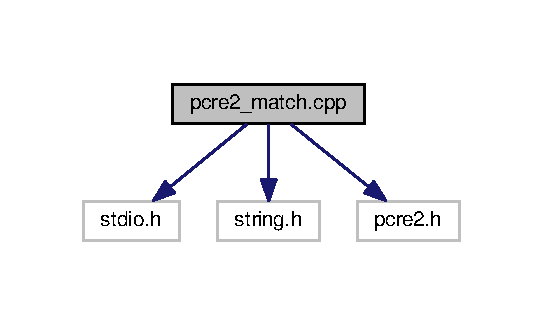
\includegraphics[width=261pt]{pcre2__match_8cpp__incl}
\end{center}
\end{figure}
\subsubsection*{Macros}
\begin{DoxyCompactItemize}
\item 
\#define \hyperlink{pcre2__match_8cpp_acff91275abcc225454675d6dfc39a58d}{P\+C\+R\+E2\+\_\+\+C\+O\+D\+E\+\_\+\+U\+N\+I\+T\+\_\+\+W\+I\+D\+TH}~8
\end{DoxyCompactItemize}
\subsubsection*{Functions}
\begin{DoxyCompactItemize}
\item 
int \hyperlink{pcre2__match_8cpp_a3c04138a5bfe5d72780bb7e82a18e627}{main} (int argc, char $\ast$$\ast$argv)
\end{DoxyCompactItemize}


\subsubsection{Macro Definition Documentation}
\hypertarget{pcre2__match_8cpp_acff91275abcc225454675d6dfc39a58d}{}\label{pcre2__match_8cpp_acff91275abcc225454675d6dfc39a58d} 
\index{pcre2\+\_\+match.\+cpp@{pcre2\+\_\+match.\+cpp}!P\+C\+R\+E2\+\_\+\+C\+O\+D\+E\+\_\+\+U\+N\+I\+T\+\_\+\+W\+I\+D\+TH@{P\+C\+R\+E2\+\_\+\+C\+O\+D\+E\+\_\+\+U\+N\+I\+T\+\_\+\+W\+I\+D\+TH}}
\index{P\+C\+R\+E2\+\_\+\+C\+O\+D\+E\+\_\+\+U\+N\+I\+T\+\_\+\+W\+I\+D\+TH@{P\+C\+R\+E2\+\_\+\+C\+O\+D\+E\+\_\+\+U\+N\+I\+T\+\_\+\+W\+I\+D\+TH}!pcre2\+\_\+match.\+cpp@{pcre2\+\_\+match.\+cpp}}
\paragraph{\texorpdfstring{P\+C\+R\+E2\+\_\+\+C\+O\+D\+E\+\_\+\+U\+N\+I\+T\+\_\+\+W\+I\+D\+TH}{PCRE2\_CODE\_UNIT\_WIDTH}}
{\footnotesize\ttfamily \#define P\+C\+R\+E2\+\_\+\+C\+O\+D\+E\+\_\+\+U\+N\+I\+T\+\_\+\+W\+I\+D\+TH~8}



\subsubsection{Function Documentation}
\hypertarget{pcre2__match_8cpp_a3c04138a5bfe5d72780bb7e82a18e627}{}\label{pcre2__match_8cpp_a3c04138a5bfe5d72780bb7e82a18e627} 
\index{pcre2\+\_\+match.\+cpp@{pcre2\+\_\+match.\+cpp}!main@{main}}
\index{main@{main}!pcre2\+\_\+match.\+cpp@{pcre2\+\_\+match.\+cpp}}
\paragraph{\texorpdfstring{main()}{main()}}
{\footnotesize\ttfamily int main (\begin{DoxyParamCaption}\item[{int}]{argc,  }\item[{char $\ast$$\ast$}]{argv }\end{DoxyParamCaption})}


\hypertarget{test__match_8cpp}{}\subsection{test\+\_\+match.\+cpp File Reference}
\label{test__match_8cpp}\index{test\+\_\+match.\+cpp@{test\+\_\+match.\+cpp}}


An example of performing regex match against a pattern with J\+P\+C\+R\+E2 and getting the match count and match results.  


{\ttfamily \#include $<$iostream$>$}\\*
{\ttfamily \#include \char`\"{}jpcre2.\+hpp\char`\"{}}\\*
Include dependency graph for test\+\_\+match.\+cpp\+:\nopagebreak
\begin{figure}[H]
\begin{center}
\leavevmode
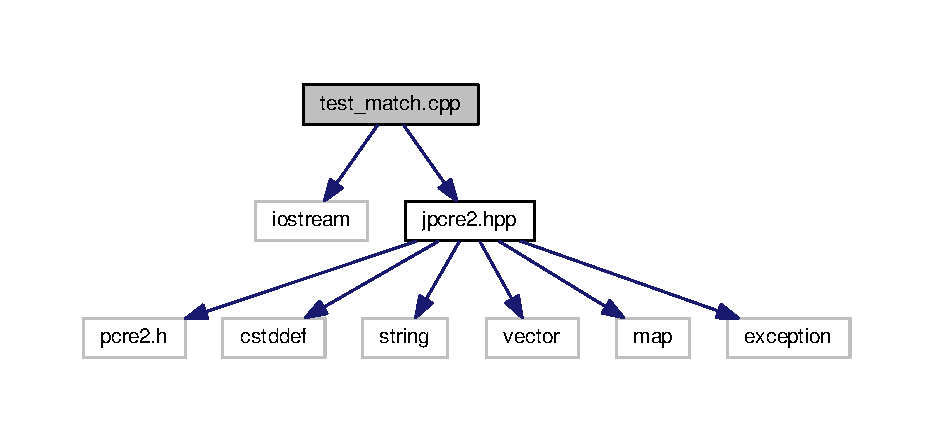
\includegraphics[width=350pt]{test__match_8cpp__incl}
\end{center}
\end{figure}


\subsubsection{Detailed Description}
An example of performing regex match against a pattern with J\+P\+C\+R\+E2 and getting the match count and match results. 

Shows how to iterate over the match results to get the captured groups/substrings. 
\begin{DoxyCodeInclude}
\textcolor{comment}{/**@file test\_match.cpp}
\textcolor{comment}{ * An example of performing regex match against a pattern with JPCRE2 and getting the}
\textcolor{comment}{ * match count and match results.}
\textcolor{comment}{ * Shows how to iterate over the match results to get the captured groups/substrings.}
\textcolor{comment}{ * @include test\_match.cpp}
\textcolor{comment}{ * @author [Md Jahidul Hamid](https://github.com/neurobin)}
\textcolor{comment}{ * */}

\textcolor{preprocessor}{#include <iostream>}
\textcolor{preprocessor}{#include "\hyperlink{jpcre2_8hpp}{jpcre2.hpp}"}


\textcolor{keywordtype}{int} main()\{

    \hyperlink{namespacejpcre2_ac1cf752c8fbb0be78020be3b80e77ce3}{jpcre2::VecNum} vec\_num0;   \textcolor{comment}{///Vector to store numbered substring Maps.}
\textcolor{comment}{}    \hyperlink{namespacejpcre2_a2b121ae776ea5b2913839f418a7d856b}{jpcre2::VecNas} vec\_nas0;   \textcolor{comment}{///Vector to store named substring Maps.}
\textcolor{comment}{}    \hyperlink{namespacejpcre2_a88a7aaf84cad627d34c8152e726168eb}{jpcre2::VecNtN} vec\_nn0;    \textcolor{comment}{///Vector to store Named substring to Number Maps.}
\textcolor{comment}{}    
    \hyperlink{classjpcre2_1_1Regex}{jpcre2::Regex} re;     \textcolor{comment}{///It's not supposed to throw any exception.}
\textcolor{comment}{}    \textcolor{comment}{}
\textcolor{comment}{    ///Compile the pattern}
\textcolor{comment}{}    \textcolor{keywordflow}{try}\{re.\hyperlink{classjpcre2_1_1Regex_a85d9a514ea86ae68533223adac6c6bd8}{setPattern}(\textcolor{stringliteral}{"(?:(?<word>[?.#@:]+)|(?<word>\(\backslash\)\(\backslash\)w+))\(\backslash\)\(\backslash\)s*(?<digit>\(\backslash\)\(\backslash\)d+)"})  \textcolor{comment}{//set pattern}
          .\hyperlink{classjpcre2_1_1Regex_aed9865b58c60945e19f36fa310f5a595}{setModifier}(\textcolor{stringliteral}{"nJ"})                                                    \textcolor{comment}{//set modifier}
          .\hyperlink{classjpcre2_1_1Regex_a03974fa7ba8f7c47186cb8d6f54934de}{addJpcre2Option}(\hyperlink{namespacejpcre2_a85c143271501e383843f45b9999c2f00a9124b768bcae4d51430aa7f26126f387}{jpcre2::VALIDATE\_MODIFIER}               
                   \textcolor{comment}{//modifier goes through validation check}
                            | \hyperlink{namespacejpcre2_a85c143271501e383843f45b9999c2f00a5e8bab7c478015b19baf3e84ed00876e}{jpcre2::JIT\_COMPILE}                               \textcolor{comment}{//
      perform JIT compile (warning if JIT is not available)}
                            | \hyperlink{namespacejpcre2_a85c143271501e383843f45b9999c2f00a6fec35fc9fdd8a606bed430c1816c552}{jpcre2::ERROR\_ALL})                                \textcolor{comment}{//treat
       warnings as errors}
          .\hyperlink{classjpcre2_1_1Regex_a2c7dcf12f26b2b046e147b013c8b5087}{addPcre2Option}(0)                                                    \textcolor{comment}{//add pcre2
       option}
          .\hyperlink{classjpcre2_1_1Regex_aad1d5ef1e87f762f68a587eec4022e69}{compile}();\}                                                          \textcolor{comment}{//Finally compile
       it.}
    \textcolor{keywordflow}{catch}(\textcolor{keywordtype}{int} e)\{std::cerr<<re.\hyperlink{classjpcre2_1_1Regex_a92b75c438ccff871205b2175a6141fd5}{getErrorMessage}(e);\}
    \textcolor{comment}{}
\textcolor{comment}{    /// The above `jpcre2::VALIDATE\_MODIFIER` option won't have any effect as modifier was passe before it.}
\textcolor{comment}{    /// You can pass a modifier (~ or &) to turn this validation check on. In that case}
\textcolor{comment}{    /// validation will start after ~ or & modifier is encountered,}
\textcolor{comment}{}
    \textcolor{comment}{/******************************************************************************************************
      *********}
\textcolor{comment}{     * Always use try catch to catch any exception and avoid unexpected termination of the program.}
\textcolor{comment}{     * All jpcre2 exceptions are of type int (integer)}
\textcolor{comment}{     * ****************************************************************************************************
      *********/}
    \textcolor{comment}{}
\textcolor{comment}{    ///subject string}
\textcolor{comment}{}    std::string subject = \textcolor{stringliteral}{"(I am a string with words and digits 45 and specials chars: ?.#@ 443 অ আ ক খ গ ঘ
        56)"};
    
    \textcolor{keywordtype}{size\_t} count=0;
    
    \textcolor{keywordflow}{try}\{count = re.\hyperlink{classjpcre2_1_1Regex_a519b0915bf1163c6ce6a4d674b30cfcd}{initMatch}()                                  \textcolor{comment}{//Invoke the initMatch() function}
                  .\hyperlink{classjpcre2_1_1RegexMatch_a9df7e92f96b61553f62720cb8f5f23e5}{setModifier}(\textcolor{stringliteral}{"gf"})                            \textcolor{comment}{//set various parameters (f:
       invalid modifier)}
                  .\hyperlink{classjpcre2_1_1RegexMatch_a635c652195deaa8ebb9e107c4f972aab}{setSubject}(subject)                          \textcolor{comment}{//...}
                  .\hyperlink{classjpcre2_1_1RegexMatch_a2c7efe1ec2e13827f670db4ecedcd0a0}{setNumberedSubstringVector}(&vec\_num0)        \textcolor{comment}{//...}
                  .\hyperlink{classjpcre2_1_1RegexMatch_ae495431f57cae54363331237ab21b56c}{setNamedSubstringVector}(&vec\_nas0)           \textcolor{comment}{//...}
                  .\hyperlink{classjpcre2_1_1RegexMatch_a04926e61d8b5f1d8bdf344efecd567d8}{setNameToNumberMapVector}(&vec\_nn0)           \textcolor{comment}{//...}
                  .\hyperlink{classjpcre2_1_1RegexMatch_a0a4cf8554a7e00f3cf2db34f60a43f60}{addJpcre2Option}(\hyperlink{namespacejpcre2_a85c143271501e383843f45b9999c2f00a9124b768bcae4d51430aa7f26126f387}{jpcre2::VALIDATE\_MODIFIER})   \textcolor{comment}{//
      ...}
                  .\hyperlink{classjpcre2_1_1RegexMatch_aac4857cd8f5eae15b29b9afbe9023522}{addPcre2Option}(0)                            \textcolor{comment}{//...}
                  .\hyperlink{classjpcre2_1_1RegexMatch_a5868aef3a146594ea1ebef34d122bb33}{match}();\}                                    \textcolor{comment}{//Finally perform the match}
    \textcolor{keywordflow}{catch}(\textcolor{keywordtype}{int} e)\{std::cerr<<\textcolor{stringliteral}{"\(\backslash\)n"}<<re.\hyperlink{classjpcre2_1_1Regex_a92b75c438ccff871205b2175a6141fd5}{getErrorMessage}(e);\}
    
    std::cerr<<re.\hyperlink{classjpcre2_1_1Regex_a1a639ae4090b88609c03e9268faf02d8}{getWarningMessage}(); \textcolor{comment}{//(f: invalid modifier) warning}
    \textcolor{comment}{}
\textcolor{comment}{    /// re.reset(); /// re-initialize re}
\textcolor{comment}{}    
    
    std::cout<<\textcolor{stringliteral}{"\(\backslash\)nTotal number of mathces: "}<<count<<std::endl;\textcolor{comment}{}
\textcolor{comment}{    ///Now let's access the matched data}
\textcolor{comment}{}    \textcolor{comment}{}
\textcolor{comment}{    ///Each of these vectors contains maps.}
\textcolor{comment}{    ///Each element in the vector specifies a particular match}
\textcolor{comment}{    ///First match is the vector element 0, second is at index 1 and so forth}
\textcolor{comment}{    ///A map for a vector element, i.e for a match contains all of its substrings/capture groups}
\textcolor{comment}{    ///The first element of the map is capture group 0 i.e total match}
\textcolor{comment}{}    
    
    \textcolor{keywordflow}{for}(\textcolor{keywordtype}{size\_t} i=0;i<vec\_num0.size();++i)\{
        
        
        std::cout<< \textcolor{stringliteral}{"\(\backslash\)n################## Match no: "}<<i+1<<\textcolor{stringliteral}{" ####################\(\backslash\)n"};
        
        
        \textcolor{comment}{}
\textcolor{comment}{        ///This vector contains maps with number as the key and the corresponding substring as the value}
\textcolor{comment}{}        std::cout<<\textcolor{stringliteral}{"\(\backslash\)n-------------------------------------------------------------------------"};
        std::cout<< \textcolor{stringliteral}{"\(\backslash\)n--- Numbered Substrings (number: substring) for match "}<<i+1<<\textcolor{stringliteral}{" ---\(\backslash\)n"};
        \textcolor{keywordflow}{for}(jpcre2::MapNum::iterator ent=vec\_num0[i].begin();ent!=vec\_num0[i].end();++ent)\{
            std::cout<<\textcolor{stringliteral}{"\(\backslash\)n\(\backslash\)t"}<<ent->first<<\textcolor{stringliteral}{": "}<<ent->second<<\textcolor{stringliteral}{"\(\backslash\)n"};
        \}
        
        
        \textcolor{comment}{}
\textcolor{comment}{        ///This vector contains maps with name as the key and the corresponding substring as the value}
\textcolor{comment}{}        std::cout<<\textcolor{stringliteral}{"\(\backslash\)n-------------------------------------------------------------------------"};
        std::cout<< \textcolor{stringliteral}{"\(\backslash\)n--- Named Substrings (name: substring) for match "}<<i+1<<\textcolor{stringliteral}{" ---\(\backslash\)n"};
        \textcolor{keywordflow}{for}(jpcre2::MapNas::iterator ent=vec\_nas0[i].begin();ent!=vec\_nas0[i].end();++ent)\{
            std::cout<<\textcolor{stringliteral}{"\(\backslash\)n\(\backslash\)t"}<<ent->first<<\textcolor{stringliteral}{": "}<<ent->second<<\textcolor{stringliteral}{"\(\backslash\)n"};
        \}
        
        
        \textcolor{comment}{}
\textcolor{comment}{        ///This vector contains maps with name as the key and number as the value}
\textcolor{comment}{        ///i.e the number (of substring) can be accessed with the name for named substring.}
\textcolor{comment}{}        std::cout<<\textcolor{stringliteral}{"\(\backslash\)n-------------------------------------------------------------------------"};
        std::cout<< \textcolor{stringliteral}{"\(\backslash\)n--- Name to number mapping (name: number/position) for match "}<<i+1<<\textcolor{stringliteral}{" ---\(\backslash\)n"};
        \textcolor{keywordflow}{for}(jpcre2::MapNtN::iterator ent=vec\_nn0[i].begin();ent!=vec\_nn0[i].end();++ent)\{
            std::cout<<\textcolor{stringliteral}{"\(\backslash\)n\(\backslash\)t"}<<ent->first<<\textcolor{stringliteral}{": "}<<ent->second<<\textcolor{stringliteral}{"\(\backslash\)n"};
        \}
    \}
    \textcolor{keywordflow}{return} 0;
\}
\end{DoxyCodeInclude}
 \begin{DoxyAuthor}{Author}
\href{https://github.com/neurobin}{\tt Md Jahidul Hamid} 
\end{DoxyAuthor}

\hypertarget{test__match2_8cpp}{}\section{test\+\_\+match2.\+cpp File Reference}
\label{test__match2_8cpp}\index{test\+\_\+match2.\+cpp@{test\+\_\+match2.\+cpp}}
{\ttfamily \#include $<$iostream$>$}\\*
{\ttfamily \#include \char`\"{}jpcre2.\+hpp\char`\"{}}\\*
\subsection*{Macros}
\begin{DoxyCompactItemize}
\item 
\#define \hyperlink{test__match2_8cpp_a0efdcb15269092623bd8d80b8d129239}{get\+Line}(a)~std\+::getline(std\+::cin,a,\textquotesingle{}\textbackslash{}n\textquotesingle{});
\end{DoxyCompactItemize}
\subsection*{Functions}
\begin{DoxyCompactItemize}
\item 
int \hyperlink{test__match2_8cpp_ae66f6b31b5ad750f1fe042a706a4e3d4}{main} ()
\end{DoxyCompactItemize}


\subsection{Macro Definition Documentation}
\index{test\+\_\+match2.\+cpp@{test\+\_\+match2.\+cpp}!get\+Line@{get\+Line}}
\index{get\+Line@{get\+Line}!test\+\_\+match2.\+cpp@{test\+\_\+match2.\+cpp}}
\subsubsection[{\texorpdfstring{get\+Line}{getLine}}]{\setlength{\rightskip}{0pt plus 5cm}\#define get\+Line(
\begin{DoxyParamCaption}
\item[{}]{a}
\end{DoxyParamCaption}
)~std\+::getline(std\+::cin,a,\textquotesingle{}\textbackslash{}n\textquotesingle{});}\hypertarget{test__match2_8cpp_a0efdcb15269092623bd8d80b8d129239}{}\label{test__match2_8cpp_a0efdcb15269092623bd8d80b8d129239}


\subsection{Function Documentation}
\index{test\+\_\+match2.\+cpp@{test\+\_\+match2.\+cpp}!main@{main}}
\index{main@{main}!test\+\_\+match2.\+cpp@{test\+\_\+match2.\+cpp}}
\subsubsection[{\texorpdfstring{main()}{main()}}]{\setlength{\rightskip}{0pt plus 5cm}int main (
\begin{DoxyParamCaption}
{}
\end{DoxyParamCaption}
)}\hypertarget{test__match2_8cpp_ae66f6b31b5ad750f1fe042a706a4e3d4}{}\label{test__match2_8cpp_ae66f6b31b5ad750f1fe042a706a4e3d4}
Vector to store numbured substring Map.

Vector to store named substring Map.

Vector to store Named substring to Number Map.

create an object

This should not throw any exception

Compile pattern

subject string

Now let\textquotesingle{}s access the matched data

Each of these vectors contains a map and each of the maps contains all the substrings that are matched against the pattern. All the matches in all the maps combines the total match throughout the entire string.

This vector contains maps with number as the key and the corresponding substring as the value

This vector contains maps with name as the key and the corresponding substring as the value

This vector contains maps with name as the key and number as the value i.\+e the number (of substring) can be accessed with the name for named substring. 
\hypertarget{test__replace_8cpp}{}\subsection{test\+\_\+replace.\+cpp File Reference}
\label{test__replace_8cpp}\index{test\+\_\+replace.\+cpp@{test\+\_\+replace.\+cpp}}


An example of doing regex replace with J\+P\+C\+R\+E2.  


{\ttfamily \#include $<$iostream$>$}\\*
{\ttfamily \#include \char`\"{}jpcre2.\+hpp\char`\"{}}\\*
Include dependency graph for test\+\_\+replace.\+cpp\+:\nopagebreak
\begin{figure}[H]
\begin{center}
\leavevmode
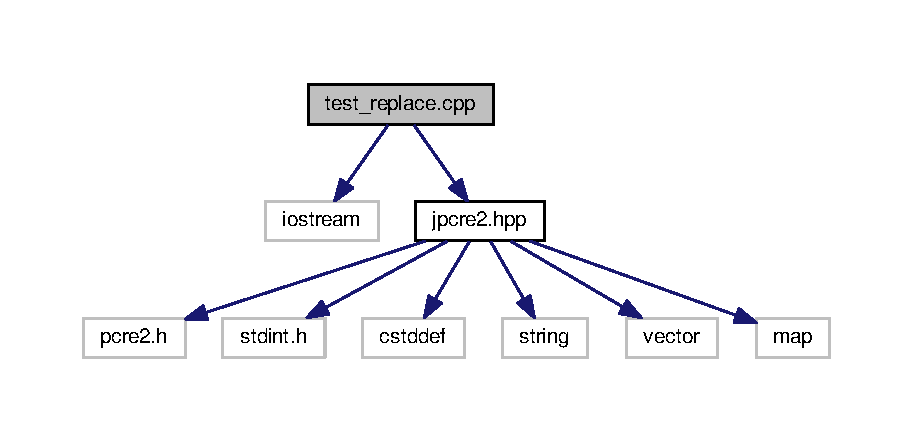
\includegraphics[width=350pt]{test__replace_8cpp__incl}
\end{center}
\end{figure}


\subsubsection{Detailed Description}
An example of doing regex replace with J\+P\+C\+R\+E2. 


\begin{DoxyCodeInclude}
\textcolor{comment}{/**@file test\_replace.cpp}
\textcolor{comment}{ * An example of doing regex replace with JPCRE2}
\textcolor{comment}{ * @include test\_replace.cpp}
\textcolor{comment}{ * @author [Md Jahidul Hamid](https://github.com/neurobin)}
\textcolor{comment}{ * */}

\textcolor{preprocessor}{#include <iostream>}
\textcolor{preprocessor}{#include "\hyperlink{jpcre2_8hpp}{jpcre2.hpp}"}


\textcolor{keywordtype}{int} main()\{
    \hyperlink{classjpcre2_1_1Regex}{jpcre2::Regex} re;     \textcolor{comment}{/// This is not supposed to throw any exception.}
\textcolor{comment}{}\textcolor{comment}{}
\textcolor{comment}{    ///Compile the pattern}
\textcolor{comment}{}    \textcolor{keywordflow}{try}\{re.\hyperlink{classjpcre2_1_1Regex_a85d9a514ea86ae68533223adac6c6bd8}{setPattern}(\textcolor{stringliteral}{"(?:(?<word>[?.#@:]+)|(?<word>\(\backslash\)\(\backslash\)w+))\(\backslash\)\(\backslash\)s*(?<digit>\(\backslash\)\(\backslash\)d+)"})     \textcolor{comment}{//Set various
       parameters}
          .\hyperlink{classjpcre2_1_1Regex_aed9865b58c60945e19f36fa310f5a595}{setModifier}(\textcolor{stringliteral}{"Jin"})                                                      \textcolor{comment}{//...}
          .\hyperlink{classjpcre2_1_1Regex_a03974fa7ba8f7c47186cb8d6f54934de}{addJpcre2Option}(\hyperlink{namespacejpcre2_a85c143271501e383843f45b9999c2f00a9124b768bcae4d51430aa7f26126f387}{jpcre2::VALIDATE\_MODIFIER})              
                      \textcolor{comment}{//...}
          .\hyperlink{classjpcre2_1_1Regex_a2c7dcf12f26b2b046e147b013c8b5087}{addPcre2Option}(0)                                                       \textcolor{comment}{//...}
          .\hyperlink{classjpcre2_1_1Regex_aad1d5ef1e87f762f68a587eec4022e69}{compile}();\}                                                             \textcolor{comment}{//Finally compile
       it.}
    \textcolor{keywordflow}{catch}(\textcolor{keywordtype}{int} e)\{std::cerr<<re.\hyperlink{classjpcre2_1_1Regex_a92b75c438ccff871205b2175a6141fd5}{getErrorMessage}(e);\}
        
    \textcolor{comment}{/******************************************************************************************************
      ************}
\textcolor{comment}{     * Use try catch block to catch any exception and avoid unexpected termination of the program in case
       of error}
\textcolor{comment}{     * All jpcre2 exceptions are of type int (integer)}
\textcolor{comment}{     * ****************************************************************************************************
      ************/}
    
    \textcolor{comment}{//subject string}
    std::string s=\textcolor{stringliteral}{"I am a string with words and digits 45 and specials chars: ?.#@ 443 অ আ ক খ গ ঘ  56"};
    
    \textcolor{keywordflow}{try}\{std::cout<<\textcolor{stringliteral}{"\(\backslash\)nreplaced string: \(\backslash\)n"}<<
        re.\hyperlink{classjpcre2_1_1Regex_ae7235a991492fa88f1bd3fb02d59cd0a}{initReplace}()                                                    \textcolor{comment}{//Invoke the
       initReplace() function}
          .\hyperlink{classjpcre2_1_1RegexReplace_a46eefdb105827920bebc8436721fa4cb}{setSubject}(s)                                                    \textcolor{comment}{//Set various
       parameters}
          .\hyperlink{classjpcre2_1_1RegexReplace_af1069f489de9b343493da2dc77b04c73}{setReplaceWith}(\textcolor{stringliteral}{"(replaced:$1)(replaced:$2)(replaced:$\{word\})"})   \textcolor{comment}{//...}
          .\hyperlink{classjpcre2_1_1RegexReplace_ae2abe2994b0fbe54950f88e63000c910}{setModifier}(\textcolor{stringliteral}{"xE"})                                                \textcolor{comment}{//...}
          .\hyperlink{classjpcre2_1_1RegexReplace_a3f86b1e11d08d0153a08244771e59061}{addJpcre2Option}(\hyperlink{namespacejpcre2_a85c143271501e383843f45b9999c2f00a9124b768bcae4d51430aa7f26126f387}{jpcre2::VALIDATE\_MODIFIER})              
               \textcolor{comment}{//...}
          .\hyperlink{classjpcre2_1_1RegexReplace_a3cfd03568b23bebcbb530a2c120b5d33}{addPcre2Option}(0)                                                \textcolor{comment}{//...}
          .\hyperlink{classjpcre2_1_1RegexReplace_afd087fa7a9bfedec802d1a3dd7edbdd0}{replace}();                                                       \textcolor{comment}{//Finally perform the
       replace operation.}
    \}
    \textcolor{keywordflow}{catch}(\textcolor{keywordtype}{int} e)\{std::cerr<<re.\hyperlink{classjpcre2_1_1Regex_a92b75c438ccff871205b2175a6141fd5}{getErrorMessage}(e);\}
    
    \textcolor{keywordflow}{return} 0;
\}
\end{DoxyCodeInclude}
 \begin{DoxyAuthor}{Author}
\href{https://github.com/neurobin}{\tt Md Jahidul Hamid} 
\end{DoxyAuthor}

\hypertarget{test__replace2_8cpp}{}\subsection{test\+\_\+replace2.\+cpp File Reference}
\label{test__replace2_8cpp}\index{test\+\_\+replace2.\+cpp@{test\+\_\+replace2.\+cpp}}


Contains an example to take subject string, replacement string, modifier and pattern from user input and perform regex replace with J\+P\+C\+R\+E2.  


{\ttfamily \#include $<$iostream$>$}\\*
{\ttfamily \#include \char`\"{}jpcre2.\+hpp\char`\"{}}\\*
Include dependency graph for test\+\_\+replace2.\+cpp\+:\nopagebreak
\begin{figure}[H]
\begin{center}
\leavevmode
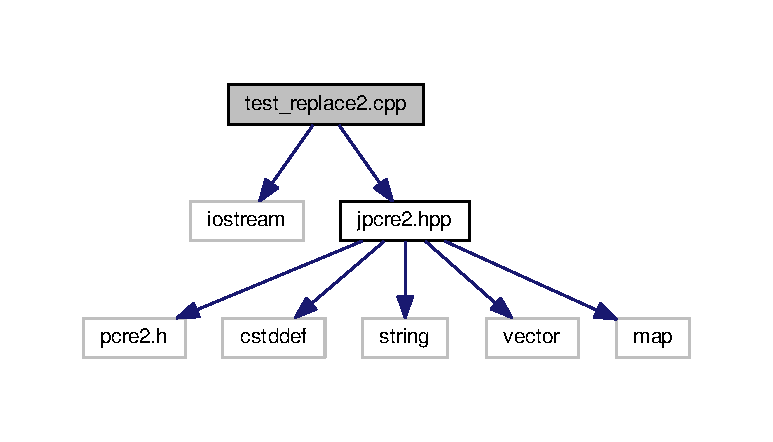
\includegraphics[width=350pt]{test__replace2_8cpp__incl}
\end{center}
\end{figure}


\subsubsection{Detailed Description}
Contains an example to take subject string, replacement string, modifier and pattern from user input and perform regex replace with J\+P\+C\+R\+E2. 


\begin{DoxyCodeInclude}
\textcolor{comment}{/**@file test\_replace2.cpp}
\textcolor{comment}{ * Contains an example to take subject string, replacement string, modifier and pattern}
\textcolor{comment}{ * from user input and perform regex replace with JPCRE2}
\textcolor{comment}{ * @include test\_replace2.cpp}
\textcolor{comment}{ * @author [Md Jahidul Hamid](https://github.com/neurobin)}
\textcolor{comment}{ * */}


\textcolor{preprocessor}{#include <iostream>}
\textcolor{preprocessor}{#include "\hyperlink{jpcre2_8hpp}{jpcre2.hpp}"}


\textcolor{preprocessor}{#define getLine(a) std::getline(std::cin,a,'\(\backslash\)n')}


\textcolor{keywordtype}{int} main()\{
    std::string pat,mod,subject,repl,repl\_mod;

    std::cout<<\textcolor{stringliteral}{"\(\backslash\)nEnter pattern: "};
    getLine(pat);

    std::cout<<\textcolor{stringliteral}{"\(\backslash\)nEnter compile modifiers (eijmnsuxADJSU): "};
    getLine(mod);
    \hyperlink{classjpcre2_1_1Regex}{jpcre2::Regex} re;     \textcolor{comment}{/// This is not supposed to throw any exception.}
\textcolor{comment}{}
\textcolor{comment}{}
\textcolor{comment}{    /// Compile the pattern}
\textcolor{comment}{}    \textcolor{keywordflow}{try}\{re.\hyperlink{classjpcre2_1_1Regex_aad1d5ef1e87f762f68a587eec4022e69}{compile}(pat,mod);\}
    \textcolor{keywordflow}{catch}(\textcolor{keywordtype}{int} e)\{std::cerr<<re.\hyperlink{classjpcre2_1_1Regex_a92b75c438ccff871205b2175a6141fd5}{getErrorMessage}(e);\}


    \textcolor{comment}{/******************************************************************************************************
      *********}
\textcolor{comment}{     * Use try catch block to catch any exception and avoid unexpected termination of the program in case
       of error.}
\textcolor{comment}{     * All jpcre2 exceptions are of type int (integer)}
\textcolor{comment}{     * ****************************************************************************************************
      *********/}

\textcolor{comment}{}
\textcolor{comment}{    ///subject string}
\textcolor{comment}{}    std::cout<<\textcolor{stringliteral}{"\(\backslash\)nEnter subject string (enter quit to quit): "}<<std::endl;
    getLine(subject);
    \textcolor{keywordflow}{if}(subject==\textcolor{stringliteral}{"quit"})\textcolor{keywordflow}{return} 0;\textcolor{comment}{}
\textcolor{comment}{     ///replacement string}
\textcolor{comment}{}    std::cout<<\textcolor{stringliteral}{"\(\backslash\)nEnter replacement string: "}<<std::endl;
    getLine(repl);
\textcolor{comment}{}
\textcolor{comment}{    /// Continue loop as long as error occurs}
\textcolor{comment}{}    \textcolor{keywordflow}{while}(\textcolor{keyword}{true})\{
        std::cout<<\textcolor{stringliteral}{"\(\backslash\)nEnter action (replacement) modifiers (eEgx): "};
        getLine(repl\_mod);

        \textcolor{comment}{//perform replace}

        \textcolor{keywordflow}{try}\{std::cout<<\textcolor{stringliteral}{"\(\backslash\)nreplaced string: "}<<re.\hyperlink{classjpcre2_1_1Regex_ae7235a991492fa88f1bd3fb02d59cd0a}{initReplace}()
                                                .\hyperlink{classjpcre2_1_1RegexReplace_a46eefdb105827920bebc8436721fa4cb}{setSubject}(subject)
                                                .\hyperlink{classjpcre2_1_1RegexReplace_af1069f489de9b343493da2dc77b04c73}{setReplaceWith}(repl)
                                                .\hyperlink{classjpcre2_1_1RegexReplace_a3f86b1e11d08d0153a08244771e59061}{addJpcre2Option}(
      \hyperlink{namespacejpcre2_a85c143271501e383843f45b9999c2f00a9124b768bcae4d51430aa7f26126f387}{jpcre2::VALIDATE\_MODIFIER})
                                                .\hyperlink{classjpcre2_1_1RegexReplace_a06a57430f62058822d48722a2a6425d7}{addModifier}(repl\_mod)
                                                .\hyperlink{classjpcre2_1_1RegexReplace_afd087fa7a9bfedec802d1a3dd7edbdd0}{replace}();\}
        \textcolor{keywordflow}{catch}(\textcolor{keywordtype}{int} e)\{std::cerr<<re.\hyperlink{classjpcre2_1_1Regex_a92b75c438ccff871205b2175a6141fd5}{getErrorMessage}(e);
            \textcolor{keywordflow}{if}(e==\hyperlink{namespacejpcre2_1_1ERROR_a4b2998984439438fa9da8d7043909bc2a4115340549b623f4e2da285bf0aa9bff}{jpcre2::ERROR::INVALID\_MODIFIER}) \textcolor{keywordflow}{continue};
        \}
        \textcolor{keywordflow}{break};
    \}
    std::cout<<\textcolor{stringliteral}{"\(\backslash\)n\(\backslash\)n--------------------------------------------------\(\backslash\)n"};
    \textcolor{comment}{//main();}
    \textcolor{keywordflow}{return} 0;
\}
\end{DoxyCodeInclude}
 \begin{DoxyAuthor}{Author}
\href{https://github.com/neurobin}{\tt Md Jahidul Hamid} 
\end{DoxyAuthor}

\hypertarget{test__shorts_8cpp}{}\section{test\+\_\+shorts.\+cpp File Reference}
\label{test__shorts_8cpp}\index{test\+\_\+shorts.\+cpp@{test\+\_\+shorts.\+cpp}}
{\ttfamily \#include $<$iostream$>$}\\*
{\ttfamily \#include \char`\"{}jpcre2.\+cpp\char`\"{}}\\*
\subsection*{Functions}
\begin{DoxyCompactItemize}
\item 
int \hyperlink{test__shorts_8cpp_ae66f6b31b5ad750f1fe042a706a4e3d4}{main} ()
\end{DoxyCompactItemize}


\subsection{Function Documentation}
\index{test\+\_\+shorts.\+cpp@{test\+\_\+shorts.\+cpp}!main@{main}}
\index{main@{main}!test\+\_\+shorts.\+cpp@{test\+\_\+shorts.\+cpp}}
\subsubsection[{\texorpdfstring{main()}{main()}}]{\setlength{\rightskip}{0pt plus 5cm}int main (
\begin{DoxyParamCaption}
{}
\end{DoxyParamCaption}
)}\hypertarget{test__shorts_8cpp_ae66f6b31b5ad750f1fe042a706a4e3d4}{}\label{test__shorts_8cpp_ae66f6b31b5ad750f1fe042a706a4e3d4}
Check if string matches the pattern

The following uses a temporary Regex object.

The above is a good example of using temporary objects to perform match (or replace)

Using the modifier S (i.\+e jpcre2\+::\+J\+I\+T\+\_\+\+C\+O\+M\+P\+I\+LE) with temporary object may or may not give you any performance boost (depends on the complexity of the pattern). The more complex the pattern gets, the more sense the S modifier makes.

If you want to match all and get the match count, use the action modifier \textquotesingle{}g\textquotesingle{}\+:

Modifiers passed to the Regex constructor or with compile() function are compile modifiers Modifiers passed with the match() or replace() functions are action modifiers

Substrings/\+Captured groups\+:

$\ast$$\ast$$\ast$ Getting captured groups/substring $\ast$$\ast$$\ast$

captured groups or substrings are stored in maps for each match, and each match is stored in a vector. Thus captured groups are in a vector of maps.

P\+C\+R\+E2 provides two types of substrings\+:
\begin{DoxyEnumerate}
\item numbered (index) substring
\item named substring
\end{DoxyEnumerate}

For the above two, we have two vectors respectively\+:
\begin{DoxyEnumerate}
\item jpcre2\+::\+Vec\+Num (Corresponding map\+: jpcre2\+::\+Map\+Num)
\item jpcre2\+::\+Vec\+Nas (Corresponding map\+: jpcre2\+::\+Map\+Nas)
\end{DoxyEnumerate}

Another additional vector is available to get the substring position/number for a particular captured group by name. It\textquotesingle{}s a vector of name to number maps
\begin{DoxyItemize}
\item jpcre2\+::\+Vec\+NtN (Corresponding map\+: jpcre2\+:Map\+NtN)
\end{DoxyItemize}

$\ast$$\ast$$\ast$$\ast$$\ast$ Get numbered substring $\ast$$\ast$$\ast$$\ast$$\ast$ ///

count (the return value) is guaranteed to give you the correct number of matches, while vec\+\_\+num.\+size() may give you wrong result if any match result was failed to be inserted in the vector. This should not happen i.\+e count and vec\+\_\+num.\+size() should always be equal.

Now vec\+\_\+num is populated with numbered substrings for each match The size of vec\+\_\+num is the total match count vec\+\_\+num\mbox{[}0\mbox{]} is the first match The type of vec\+\_\+num\mbox{[}0\mbox{]} is jpcre2\+::\+Map\+Num

Total match (group 0) from first match

captured group 1 from first match

captured group 2 from first match

captured group 3 doesn\textquotesingle{}t exist, it will give you empty string

Using the \mbox{[}\mbox{]} operator with jpcre2\+::\+Map\+Num will create new element if it doesn\textquotesingle{}t exist i.\+e vec\+\_\+num\mbox{[}0\mbox{]}\mbox{[}3\mbox{]} were created in the above example. This should be ok, if existence of a particular substring is not important

If the existence of a substring is important, use the std\+::map\+::find() or std\+::map\+::at() ($>$=C++11) function to access map elements

There were two matches found (vec\+\_\+num.\+size() == 2) in the above example

Total match (group 0) from second match

captured group 1 from second match

captured group 2 from second match

$\ast$$\ast$$\ast$$\ast$$\ast$ Get named substring $\ast$$\ast$$\ast$$\ast$$\ast$ ///

We will get name to number map vector too

.set\+Numbered\+Substring\+Vector(vec\+\_\+num) /// We don\textquotesingle{}t need it in this example

Additional (name to number maps)

Now vec\+\_\+nas is populated with named substrings for each match The size of vec\+\_\+nas is the total match count vec\+\_\+nas\mbox{[}0\mbox{]} is the first match The type of vec\+\_\+nas\mbox{[}0\mbox{]} is jpcre2\+::\+Map\+Nas

If the existence of a substring is important, use the std\+::map\+::find() or std\+::map\+::at() ($>$=C++11) function to access map elements

There were two matches found (vec\+\_\+nas.\+size() == 2) in the above example

Get the position (number) of a captured group name (that was found in match)

Replacement Examples Replace pattern in a string with a replacement string

The init\+Replace() function can take a subject and replacement string as argument. You can also pass the subject with set\+Subject() function in method chain, replacement string with set\+Replace\+With() function in method chain, etc ...

A call to replace() will return the resultant string

replace first occurrence of a digit with @

replace all occrrences of a digit with @

swap two parts of a string 
%--- End generated contents ---

% Index
\backmatter
\newpage
\phantomsection
\clearemptydoublepage
\addcontentsline{toc}{chapter}{Index}
\printindex

\end{document}
